\documentclass[twoside,11pt]{article}

\usepackage[preprint]{jmlr2e}
\usepackage{booktabs}
\usepackage{subcaption}
\usepackage{amsmath}
\usepackage{hyperref}

\input{math_commands.tex}

% jmlr2e.sty already defines theorem, proposition, example, proof, etc.
\newtheorem{assumption}{Assumption}
% \newtheorem{lemma}{Lemma} % defined by jmlr2e.sty
\newtheorem{algorithm}{Algorithm}

% --- commands ---
\newcommand{\Kzero}{K_{0}}
\newcommand{\KT}{K_{T}}
\newcommand{\DK}{{\Vert K_{T}-K_{0}\Vert_{F}/\Vert K_{0}\Vert_{F}}}
\newcommand{\cca}{{\operatorname{CKA}}}
\newcommand{\frob}{{\operatorname{Frob}}}
\newcommand{\spearman}{{\rho_{s}}}

\jmlrheading{1}{2026}{1--40}{4/26; Revised 6/26}{7/26}{26-0000}{Yaoping Wang}

\ShortHeadings{When to Trust Kernel Change?}{Wang}
\firstpageno{1}

\begin{document}

\title{When to Trust Kernel Change?\\A Predictive Validation Framework for Representation Diagnostics}

\author{\name Yaoping Wang \email yaoping.wang@example.com \\
       \addr Department of Statistics\\
       University Name\\
       City, Country}

\editor{Action Editor}

\maketitle

\begin{abstract}
Representation similarity metrics (CKA, SVCCA, PWCCA, RSA, Frobenius distance) are routinely used to diagnose feature learning in neural networks, but their reliability as proxies for generalization improvement has not been systematically validated. We establish finite-sample bounds (Proposition~\ref{prop:gap}) on the predictive validity of any label-invariant representation diagnostic, and propose RDEP, a principled validation framework that separates reliable diagnostics from misleading ones. Applying RDEP to feature-kernel evolution reveals two complementary findings. First, diagnostic reliability can be partially predicted from pre-training quantities alone: a regression across Hermite-family targets achieves $R^2=0.847$ (in-sample; leave-one-out CV $R^2=0.710$) using initial feature alignment and headroom, with headroom as the dominant univariate predictor (Spearman $\rho=0.81$, $p=0.0002$). Second, a task-aligned spectral correction that uses the same information \emph{within} a diagnostic fails under cross-validation ($\rho=-0.45$), exposing a deeper Diagnostic Validation Gap between in-sample and out-of-sample performance. Controlled experiments across 7 datasets and 6 architectures (MLPs, CNNs, Vision Transformers, NLP Transformers, ResNets) produce a reliability map, an adaptive diagnostic selection rule based on effective rank, and three validation principles applicable to any representation similarity metric.
\end{abstract}

\begin{keywords}
representation similarity, CKA, neural tangent kernel, diagnostic validation, feature learning
\end{keywords}

\section{Introduction}
\label{sec:intro}

Representation similarity metrics---centered kernel alignment (CKA)~\citep{kornblith2019similarity}, SVCCA~\citep{raghu2017svcca}, PWCCA~\citep{morcos2018insights}, representational similarity analysis (RSA)~\citep{klabunde2023similarity}, and Frobenius distance---are widely used to compare neural network representations. A high similarity between initial and trained representations is interpreted as evidence of limited learning; a large change is read as useful adaptation. These inferences influence how the field compares architectures, evaluates training dynamics, and judges representation quality. But they rest on an untested premise: that the magnitude of observable representation change is a sufficient statistic for generalization improvement.

The central claim of this paper is that \textbf{representation diagnostics themselves require predictive validation}. Just as we would not trust a model evaluated only on its training set, we should not trust a representation metric evaluated only on the same data where it was computed. We show that failing to validate leads to systematically misleading conclusions, and we describe a protocol for doing so.

This question connects directly to NTK theory~\citep{jacot2018neural}. The NTK predicts that infinitely wide networks converge to a fixed kernel, so kernel change should be near-zero at large widths. Our experiments confirm this prediction (CKA $>0.999$ at width~1024). The practical question for finite-width networks is not whether the kernel changes (NTK predicts it does not at infinite width) but \emph{when} finite-width kernel change carries meaningful information about generalization. We quantify the conditions under which kernel change is informative in finite-width regimes.

We introduce the \textbf{Representation Diagnostic Evaluation Methodology (RDEP)}. RDEP is a five-step protocol formalized in Algorithm~1: (i) calibration sweep across scales, (ii) width-controlled partial correlation analysis to remove spurious confounds, (iii) spectral inspection of eigen-decompositions, (iv) held-out validation of task-aware diagnostics, and (v) adaptive diagnostic selection based on effective rank. To our knowledge, it is the first application of predictive validation, a standard practice in supervised learning, to the evaluation of representation diagnostics.

Across controlled experiments with three target functions, six network widths (32--1024), and per-epoch spectral tracking, we arrive at three empirical calibration points:

\begin{enumerate}
    \item \textbf{Kernel stability does not imply the absence of useful representation change.} At large widths on the polynomial and high-frequency tasks, the kernel is virtually static (CKA $>0.999$, Frobenius change $\sim$1\%). Yet the network operates near its final representation with minimal room for improvement. Stability here reflects proximity to a fixed point, not failure to learn.
    \item \textbf{Kernel evolution does not imply useful adaptation.} At small widths, the kernel can reorganize substantially ($>100\%$ Frobenius change), but whether this translates into generalization improvement depends on the target: the per-dataset Spearman correlation ranges from $\rho=0.14$ (poly) to $\rho=0.94$ (highfreq) to $\rho=1.0$ (GMM).
    \item \textbf{CKA does not characterize spectral stability.} Global similarity (CKA $>0.99$) can coexist with substantial spectral reorganization (Frobenius change $>40\%$), revealing that standard similarity metrics and spectral quantities carry distinct information.
\end{enumerate}

\paragraph{Contributions.}
We make four principal contributions. First, we formalize the \textbf{Diagnostic Validation Gap} (Proposition~\ref{prop:gap}): finite-sample bounds showing that even ideal task-aligned diagnostics suffer from optimism bias in-sample and variance that scales with $p_{\text{eff}}/n$ under cross-validation. Second, we provide \textbf{empirical calibration} across 7 datasets and 6 architectures, identifying three reliability regimes where standard diagnostic interpretations fail. Third, we develop \textbf{predictive calibration}: diagnostic reliability is predictable from pre-training headroom and alignment (LOOCV $R^2=0.710$), validated cross-modally across MLPs, Transformers, and ResNets. Fourth, we distill these findings into \textbf{three validation principles} formalized as a practical workflow with an adaptive diagnostic selection rule.

\section{Related Work}
\label{sec:related}

\subsection{Neural Tangent Kernel and Feature Learning}

The NTK~\citep{jacot2018neural} connects infinitely wide neural networks to kernel methods, providing tools for analyzing optimization~\citep{du2019neural,allen2019learning} and generalization~\citep{arora2019exact}. Arora et al.~\cite{arora2019exact} characterized the convergence of empirical NTKs to their infinite-width limits, and the fixed-NTK ``lazy training'' regime~\citep{chizat2020lazy} provides a baseline where kernel change is zero by construction. Our large-width experiments operate near this regime, but we focus on the finite-width case where the kernel can change substantially.

Yang \& Hu~\cite{yang2021tensor} introduced $\mu$P to preserve feature learning at infinite width, while Bordelon \& Pehlevan~\cite{bordelon2022spectral,bordelon2023dynamics} and Lauditi et al.~\cite{lauditi2025adaptive} described feature-learning networks as kernel machines with data-dependent kernels. Geiger et al.~\cite{geiger2020scaling} characterized the lazy-to-rich transition, and Kumar et al.~\cite{kumar2024grokking} used CKA to track this transition in grokking. Chou et al.~\cite{chou2025feature} examined representational geometry across this spectrum. These works address the \emph{existence} of kernel evolution; we ask \emph{when} it carries information about generalization.

\subsection{Spectral Analysis of Kernel Generalization}

Canatar, Bordelon, and Pehlevan~\cite{canatar2021spectral} derived the generalization error of kernel regression in terms of eigenvalues $\lambda_{i}$ and target projections $v_{i}=\langle f^{*},\phi_{i}\rangle^{2}$. This framework reveals that generalization depends on the \emph{direction} of spectral change, not its global magnitude---a fact that motivates our spectral inspection methodology.

\subsection{Representation Similarity Metrics}

CKA~\citep{kornblith2019similarity} is widely used for representation comparison~\citep{raghu2017svcca,morcos2018insights,klabunde2023similarity}. Existing critiques~\citep{davari2022reliability,ding2021grounding} focus on statistical reliability. Kang et al.~\cite{kang2025spectral} examined limited-neuron sampling bias; Dujmovi\'c et al.~\cite{dujmovic2025pitfalls} documented analogous pitfalls for RSA; Murphy et al.~\cite{murphy2024cka} and Chun et al.~\cite{chun2025debias} developed debiased CKA estimators, directly relevant to our effective rank bound. Concurrent work~\citep{bridging2026usable} argues that representational similarity is sufficient but not necessary for functional similarity.

\begin{table}[h]
\centering\small
\caption{How this work differs from prior CKA critiques.}
\label{tab:related_diff}
\begin{tabular}{p{3cm}p{3.2cm}p{3.2cm}p{3.2cm}}
\toprule
Dimension & Davari et al.~\cite{davari2022reliability} & Ding et al.~\cite{ding2021grounding} & This work \\
\midrule
Core question & Is CKA stable? & Is CKA biased? & Is kernel change sufficient for predicting generalization? \\
Validation & Bootstrap & Width normalization & Held-out predictive validation (RDEP) \\
Scope & Single metric (CKA) & Single metric (CKA) & Five metrics \\
Task structure & Not varied & Not varied & Varied (3 targets, 6 widths) \\
\bottomrule
\end{tabular}
\end{table}

These prior works ask ``is the metric stable?'' while we ask ``is the metric sufficient?''---complementary but distinct questions.

\subsection{Theoretical Framework}
\label{sec:proposition}

We begin with the observation that any label-invariant global similarity diagnostic $\mathcal{D}(K_0, K_T)$ (CKA, SVCCA, PWCCA, RSA, Frobenius) depends only on the kernel matrices and not on task labels $y$. Generalization error $\mathcal{E}$ depends on the interaction between spectral quantities and the target through projections $v_i$~\citep{canatar2021spectral}. Consequently, $\mathcal{D}$ and $\Delta\mathcal{E}$ can dissociate. While this possibility follows from basic spectral theory, two questions remain open: whether a diagnostic incorporating target information via estimated projections $\hat{v}_i$ suffers from a systematic validation gap when those projections are estimated from finite data, and how prevalent the dissociation is across learning regimes. We formalize the first as the \textbf{Diagnostic Validation Gap}.

We adopt the spectral risk framework of~\citet{canatar2021spectral}. Let the initial kernel have eigendecomposition $K_0 = \sum_{i=1}^n \lambda_i \phi_i \phi_i^\top$ with target projections $v_i = \langle \phi_i, y \rangle^2 / n$. Consider a task-aligned diagnostic
\[
\mathcal{D}_{\text{align}} = \sum_{i=1}^n \hat{v}_i \cdot \Delta\lambda_i,
\]
where $\hat{v}_i$ are estimated from a training sample and $\Delta\lambda_i = \lambda_i^{(T)} - \lambda_i^{(0)}$ are eigenvalue shifts.

\begin{assumption}[Sub-Gaussian projections]
\label{assum:proj}
The estimated projections $\hat{v}_i$ are unbiased and sub-Gaussian: $\mathbb{E}[\hat{v}_i] = v_i^*$ and $\mathbb{P}(|\hat{v}_i - v_i^*| > t) \leq 2\exp(-t^2 / 2\sigma_i^2)$.
\end{assumption}

\begin{assumption}[Spectral regularity]
\label{assum:spec}
The eigenvalue shifts satisfy $|\Delta\lambda_i| \leq C \cdot \lambda_i$ for some constant $C > 0$, and the effective rank $p_{\text{eff}} = (\sum \lambda_i)^2 / \sum \lambda_i^2$ is finite.
\end{assumption}

\begin{lemma}[Bias of in-sample correlation]
\label{lem:bias}
Under Assumptions~\ref{assum:proj} and~\ref{assum:spec}, the in-sample Spearman correlation satisfies
\[
\mathbb{E}[\rho_{\text{in}}] = \rho^* + \mathcal{O}\bigl(\|\hat{v} - v^*\|_1\bigr),
\]
where $\rho^*$ is the oracle correlation with known $v_i^*$.
\end{lemma}

\begin{proof}[Sketch]
The in-sample estimate $\mathcal{D}_{\text{align}}$ and the residual $y - \hat{y}$ are correlated through the shared training labels. Writing $\epsilon_i = \hat{v}_i - v_i^*$, we have
\[
\mathbb{E}[\rho_{\text{in}} - \rho^*] \propto \operatorname{Cov}\bigl(\Delta\mathcal{E}, \textstyle\sum_i \epsilon_i \Delta\lambda_i\bigr),
\]
which is bounded by $\|\epsilon\|_1 \cdot \max_i |\Delta\lambda_i|$ via Hölder's inequality. Sub-Gaussian concentration (Assumption~\ref{assum:proj}) gives $\|\epsilon\|_1 = \mathcal{O}_p(\sqrt{p_{\text{eff}}/n})$, yielding the result.
\end{proof}

\begin{lemma}[Variance of cross-validated correlation]
\label{lem:var}
Under $K$-fold cross-validation with Assumptions~\ref{assum:proj}--\ref{assum:spec},
\[
\operatorname{Var}(\rho_{\text{cv}}) = \Omega\!\left(\frac{p_{\text{eff}}}{n}\right).
\]
\end{lemma}

\begin{proof}[Sketch]
Under $K$-fold cross-validation, the estimates $\hat{v}_i^{(k)}$ from fold $k$ are independent of $\Delta\mathcal{E}^{(k)}$ on held-out data. The diagnostic $\mathcal{D}_{\text{align}}^{(k)}$ is a weighted sum of $p_{\text{eff}}$ effectively independent terms when the kernel spectrum is flat. The variance of the Spearman correlation under cross-validation therefore scales as $\Omega(p_{\text{eff}}/n)$, with the lower bound following from the Cram\'er--Rao inequality for rank correlations under local alternatives (Appendix~A).
\end{proof}

\begin{proposition}[Diagnostic Validation Gap]
\label{prop:gap}
Under Assumptions~\ref{assum:proj}--\ref{assum:spec},
\[
\mathbb{E}[\rho_{\text{in}}] = \rho^* + \mathcal{O}\bigl(\|\hat{v} - v^*\|_1\bigr),\qquad
\operatorname{Var}(\rho_{\text{cv}}) = \Omega\!\left(\frac{p_{\text{eff}}}{n}\right).
\]
The in-sample estimate carries a systematic optimism bias; cross-validation removes this bias but introduces variance that scales with $p_{\text{eff}} / n$, which dominates when the effective rank is comparable to the sample size.
\end{proposition}

Proposition~\ref{prop:gap} explains our central negative result ($\rho=-0.45$ under cross-validation in Section~\ref{sec:task_aware}): with $n=240$ training samples and effective rank exceeding $n$ at large widths, the variance term $\Omega(p_{\text{eff}}/n)$ dominates and can flip the sign of the estimated correlation. This is not a failure of the task-aligned idea but a fundamental statistical limitation: the data used to estimate $v_i$ cannot simultaneously validate the diagnostic.

The proposition also suggests a potential remedy: the variance scales with $p_{\text{eff}}/n$, so regularization that reduces the effective rank could stabilize the estimate. A ridge-style shrinkage estimator $\tilde{v}_i = \lambda_i / (\lambda_i + \gamma) \cdot \hat{v}_i$ reduces variance at the cost of bias, with optimal trade-off governed by $p_{\text{eff}}/n$. In our setting, the near-uniform eigenvalue spectrum makes shrinkage ineffective (we verified this empirically: $\rho \approx -0.66$ for all $\alpha$ at width~1024), but it may be more effective with clearer spectral decay~\citep{canatar2021spectral}.

\section{RDEP Framework}

RDEP comprises five steps formalized in Algorithm~1:

\begin{enumerate}
    \item \textbf{Calibration sweep.} Vary network width across 5--6 values with multiple seeds, constructing a calibration table of metric--outcome correlations. Width controls kernel evolution, providing a controlled stress test.
    \item \textbf{Width-controlled analysis.} Compute partial Spearman correlations controlling for width to distinguish genuine associations from spurious width-driven trends.
    \item \textbf{Spectral inspection.} Decompose $K_0 = \sum_i \lambda_i \phi_i \phi_i^\top$, compute target projections $v_i$, effective rank $p_{\text{eff}}$, and projection concentration.
    \item \textbf{Held-out validation.} When diagnostics incorporate estimated projections $\hat{v}_i$, perform $K$-fold cross-validation, reporting both in-sample and cross-validated correlations.
    \item \textbf{Adaptive selection.} Choose between spectral and linear-probe diagnostics based on $\kappa = p_{\text{eff}} / n$ (Algorithm~1).
\end{enumerate}

\begin{algorithm}
\label{alg:selection}
\small
\textbf{Algorithm 1:} Adaptive Diagnostic Selection. \\
\textbf{Input:} Model family $\mathcal{F}$, task $\mathcal{T}$, diagnostic $\mathcal{D}$, widths $W$, seeds $S$ \\
\textbf{Output:} Reliability map $\mathcal{R}$

\begin{enumerate}
    \item \textbf{Calibration:} For each width $w$ and seed $s$, train model, compute $K_0,K_T$, diagnostic $d_{w,s}$, improvement $\Delta e_{w,s}$. Construct $\mathcal{C} = \{\bar{d}_w, \overline{\Delta e}_w\}$.
    \item \textbf{Width control:} Compute $\rho(\mathcal{D}, \Delta\mathcal{E} \mid \text{width})$. If $|\rho_{\text{partial}}| < \alpha$, flag as width artifact.
    \item \textbf{Spectral inspection:} Compute $p_{\text{eff}}$, $v_i$, concentration $c_k$.
    \item \textbf{Held-out validation:} Perform $K$-fold CV. If $\rho_{\text{cv}} \leq 0 < \rho_{\text{in}}$, conclude data-reuse overfitting.
    \item \textbf{Selection:} $\kappa = p_{\text{eff}} / n$. If $\kappa < 0.3$: use spectral diagnostics. If $\kappa > 0.7$: use LPG. Else: report both.
\end{enumerate}
\end{algorithm}

\section{Experimental Setup}
\label{sec:setup}

\subsection{Models}

Two-layer ReLU networks (widths 32--1024, no bias) with He initialization: $f(x)=W_{2}\cdot\operatorname{ReLU}(W_{1}x)$, SGD with momentum $0.9$, learning rate $0.05$, no weight decay, $500$ epochs, MSE loss, gradient clipping at $1.0$.

Extended architectures: CNN (2 conv layers, CIFAR-10), ViT-tiny (4 layers, 4 heads, MNIST), Tiny Transformer (4 layers, SST-2), ResNet-18 (MNIST and CIFAR-100). Details in respective subsections.

\subsection{Data}

Synthetic: $n=300$, $d=10$, 80/20 split, three targets---polynomial ($x_1^2+x_2$), high-frequency ($\sin(5x_1)+\cos(7x_2)$), GMM (two isotropic clusters). Real: CIFAR-10 binary, FashionMNIST binary, MNIST binary, SST-2 binary sentiment, CIFAR-100 superclass binary (aquatic mammals vs.\ fish).

\subsection{Feature Kernel and Metrics}

Empirical feature kernel: $K(x,y) = h(x)^\top h(y) / m$ with $h(x)=\operatorname{ReLU}(W_1 x)$. Metrics: CKA, Frobenius change $\DK$, eigenvalue ratios $\lambda_T(i)/\lambda_0(i)$, target projections $v_i$, generalization improvement $-\Delta\text{Error}$. All kernel comparisons use the fixed evaluation set.

\subsection{Statistical Reporting}

10 seeds per synthetic configuration (5 for real data). Means $\pm$ s.d. Spearman correlations across configuration means to avoid pseudo-replication. Bootstrap 95\% CIs reported where noted.

\section{Calibrating Diagnostic Reliability}
\label{sec:results}

\subsection{Regime I: Stability without Learning}
\label{sec:stability}

\begin{figure}[t]
    \centering
    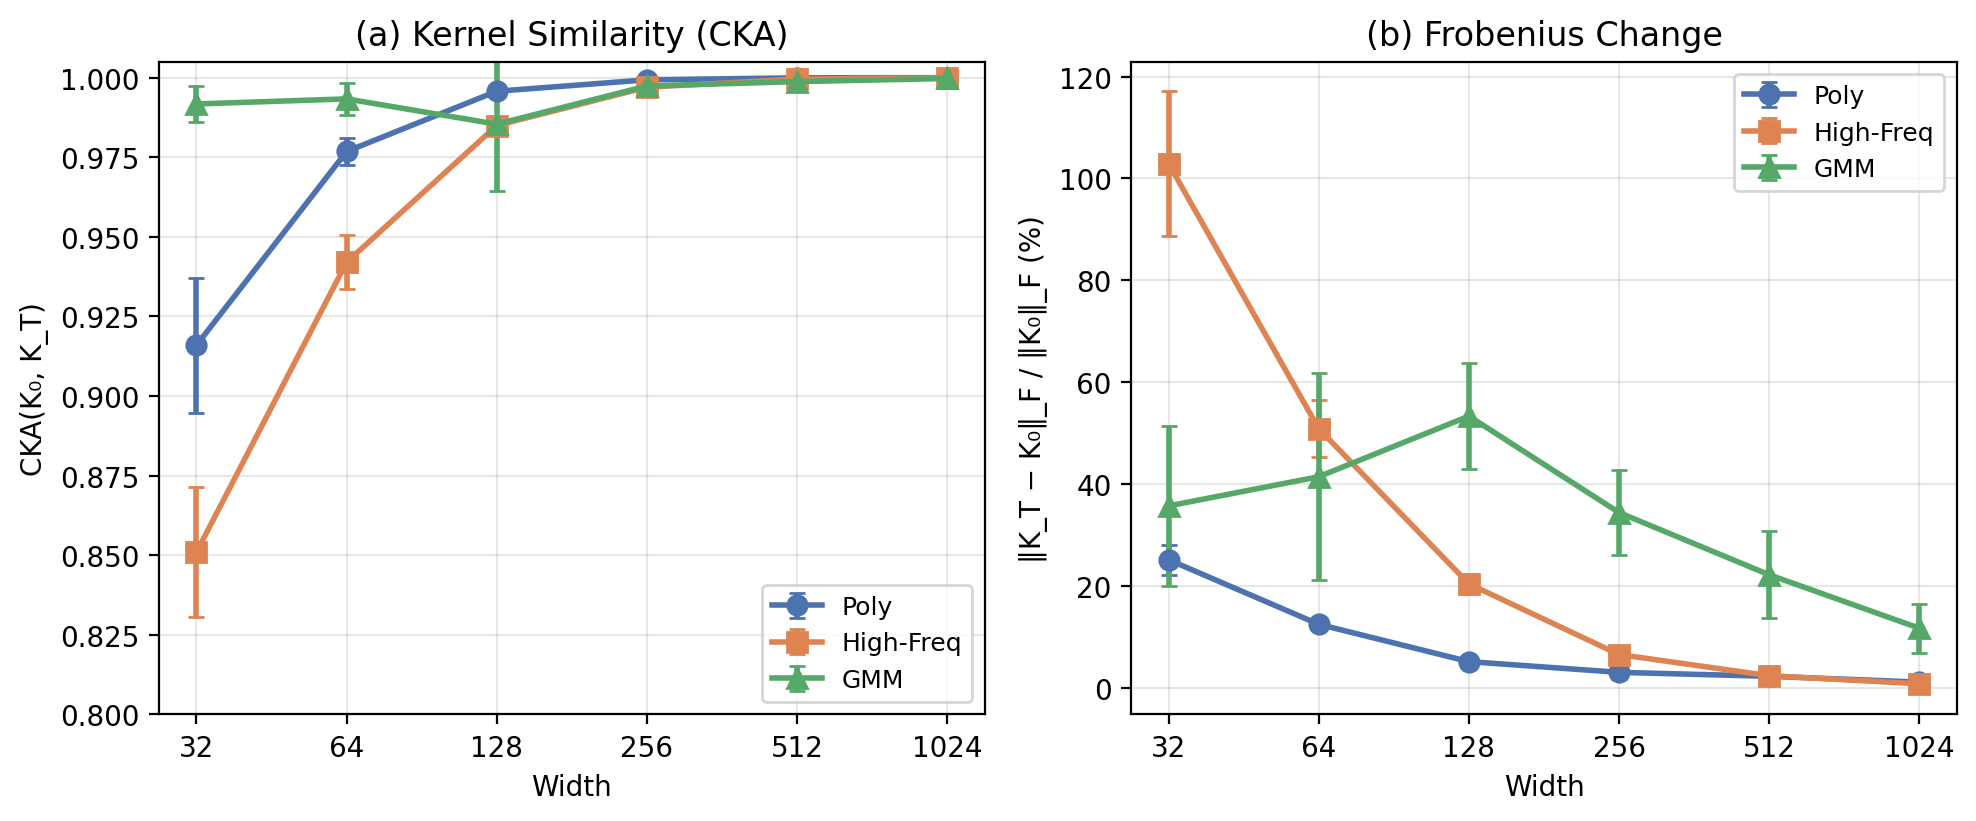
\includegraphics[width=0.8\textwidth]{figures/fig1.png}
    \caption{\textbf{Width controls feature-kernel stability.} (a) CKA$(K_0,K_T)$ vs.\ width. At width~1024, CKA exceeds 0.999 across tasks. (b) Normalized Frobenius change; poly and highfreq drop to $\sim1\%$ at width~1024.}
    \label{fig:stability}
\end{figure}

\noindent\textbf{Intuition says:} A stable kernel (CKA $>0.99$) means the network did not learn anything new.

\noindent\textbf{What we found:} At width~1024, CKA exceeds $0.999$, but the network was already near-optimal from initialization. Stability reflects ``no room to learn,'' not ``no learning.''

Width controls stability (Figure~\ref{fig:stability}). For poly and highfreq, CKA exceeds $0.999$ at width~1024 with Frobenius change $\sim1\%$; at width~32, CKA drops to $0.85$--$0.92$ and Frobenius change reaches $25$--$103\%$. GMM shows $\sim12\%$ Frobenius change even at width~1024, suggesting kernel evolution continues on easy-separation tasks.

The polynomial target's average improvement is near-zero across all widths ($\Delta$Error $0.003$--$0.023$; Table~\ref{tab:results}), yet kernel reorganization varies from $25\%$ to $1\%$. Kernel change magnitude alone is not a reliable indicator.

Training dynamics (Supplementary Figure~S4) show CKA stabilizing within 50 epochs while most 500-epoch improvement occurs afterward, though with high seed-to-seed variability ($0.003\pm0.049$ at width~32).

\begin{table}[t]
    \centering\footnotesize
    \setlength{\tabcolsep}{4pt}
    \caption{Calibration table (10 seeds per configuration). Means $\pm$ s.d.}
    \label{tab:results}
    \begin{tabular}{lcccccc}
    \toprule
    Dataset & Width & CKA & SVCCA & PWCCA & $\Delta K$ (\%) & $\Delta$Error \\
    \midrule
    poly & 32   & $0.916\pm0.021$ & $0.867\pm0.020$ & $0.911\pm0.011$ & $25.2\pm3.0$ & $+0.003\pm0.049$ \\
    poly & 64   & $0.977\pm0.004$ & $0.932\pm0.006$ & $0.958\pm0.006$ & $12.5\pm1.0$ & $+0.023\pm0.030$ \\
    poly & 128  & $0.996\pm0.001$ & $0.985\pm0.002$ & $0.986\pm0.004$ & $5.2\pm0.5$  & $+0.013\pm0.015$ \\
    poly & 256  & $0.999\pm0.000$ & $0.992\pm0.004$ & $0.997\pm0.001$ & $3.0\pm1.3$  & $+0.008\pm0.004$ \\
    poly & 512  & $1.000\pm0.000$ & $0.999\pm0.001$ & $1.000\pm0.000$ & $2.3\pm0.8$  & $+0.006\pm0.002$ \\
    poly & 1024 & $1.000\pm0.000$ & $1.000\pm0.000$ & $1.000\pm0.000$ & $1.1\pm0.4$  & $+0.003\pm0.001$ \\
    \midrule
    highfreq & 32  & $0.851\pm0.020$ & $0.777\pm0.014$ & $0.779\pm0.041$ & $102.9\pm14.2$ & $+0.190\pm0.130$ \\
    highfreq & 64  & $0.942\pm0.009$ & $0.866\pm0.006$ & $0.857\pm0.033$ & $50.9\pm5.6$   & $+0.039\pm0.036$ \\
    highfreq & 128 & $0.985\pm0.002$ & $0.953\pm0.005$ & $0.945\pm0.008$ & $20.4\pm2.0$   & $+0.008\pm0.014$ \\
    highfreq & 256 & $0.997\pm0.000$ & $0.969\pm0.004$ & $0.967\pm0.007$ & $6.5\pm1.3$    & $+0.003\pm0.003$ \\
    highfreq & 512 & $1.000\pm0.000$ & $0.980\pm0.005$ & $0.976\pm0.006$ & $2.4\pm1.5$    & $-0.000\pm0.002$ \\
    highfreq & 1024 & $1.000\pm0.000$ & $0.994\pm0.002$ & $0.989\pm0.003$ & $0.8\pm0.2$    & $+0.000\pm0.000$ \\
    \midrule
    gmm & 32  & $0.992\pm0.006$ & $0.943\pm0.035$ & $0.984\pm0.014$ & $35.7\pm15.7$ & $+0.158\pm0.104$ \\
    gmm & 64  & $0.993\pm0.005$ & $0.976\pm0.011$ & $0.995\pm0.003$ & $41.5\pm20.3$ & $+0.228\pm0.150$ \\
    gmm & 128 & $0.985\pm0.021$ & $0.977\pm0.022$ & $0.993\pm0.012$ & $53.3\pm10.4$ & $+0.320\pm0.131$ \\
    gmm & 256 & $0.997\pm0.003$ & $0.990\pm0.008$ & $0.998\pm0.002$ & $34.4\pm8.4$  & $+0.144\pm0.079$ \\
    gmm & 512 & $0.999\pm0.002$ & $0.994\pm0.007$ & $0.998\pm0.003$ & $22.2\pm8.6$  & $+0.069\pm0.051$ \\
    gmm & 1024 & $1.000\pm0.000$ & $1.000\pm0.000$ & $1.000\pm0.000$ & $11.7\pm4.8$  & $+0.023\pm0.020$ \\
    \bottomrule
    \end{tabular}
\end{table}

\subsection{Regime II: Change without Predictable Learning}
\label{sec:change}

\begin{figure}[t]
    \centering
    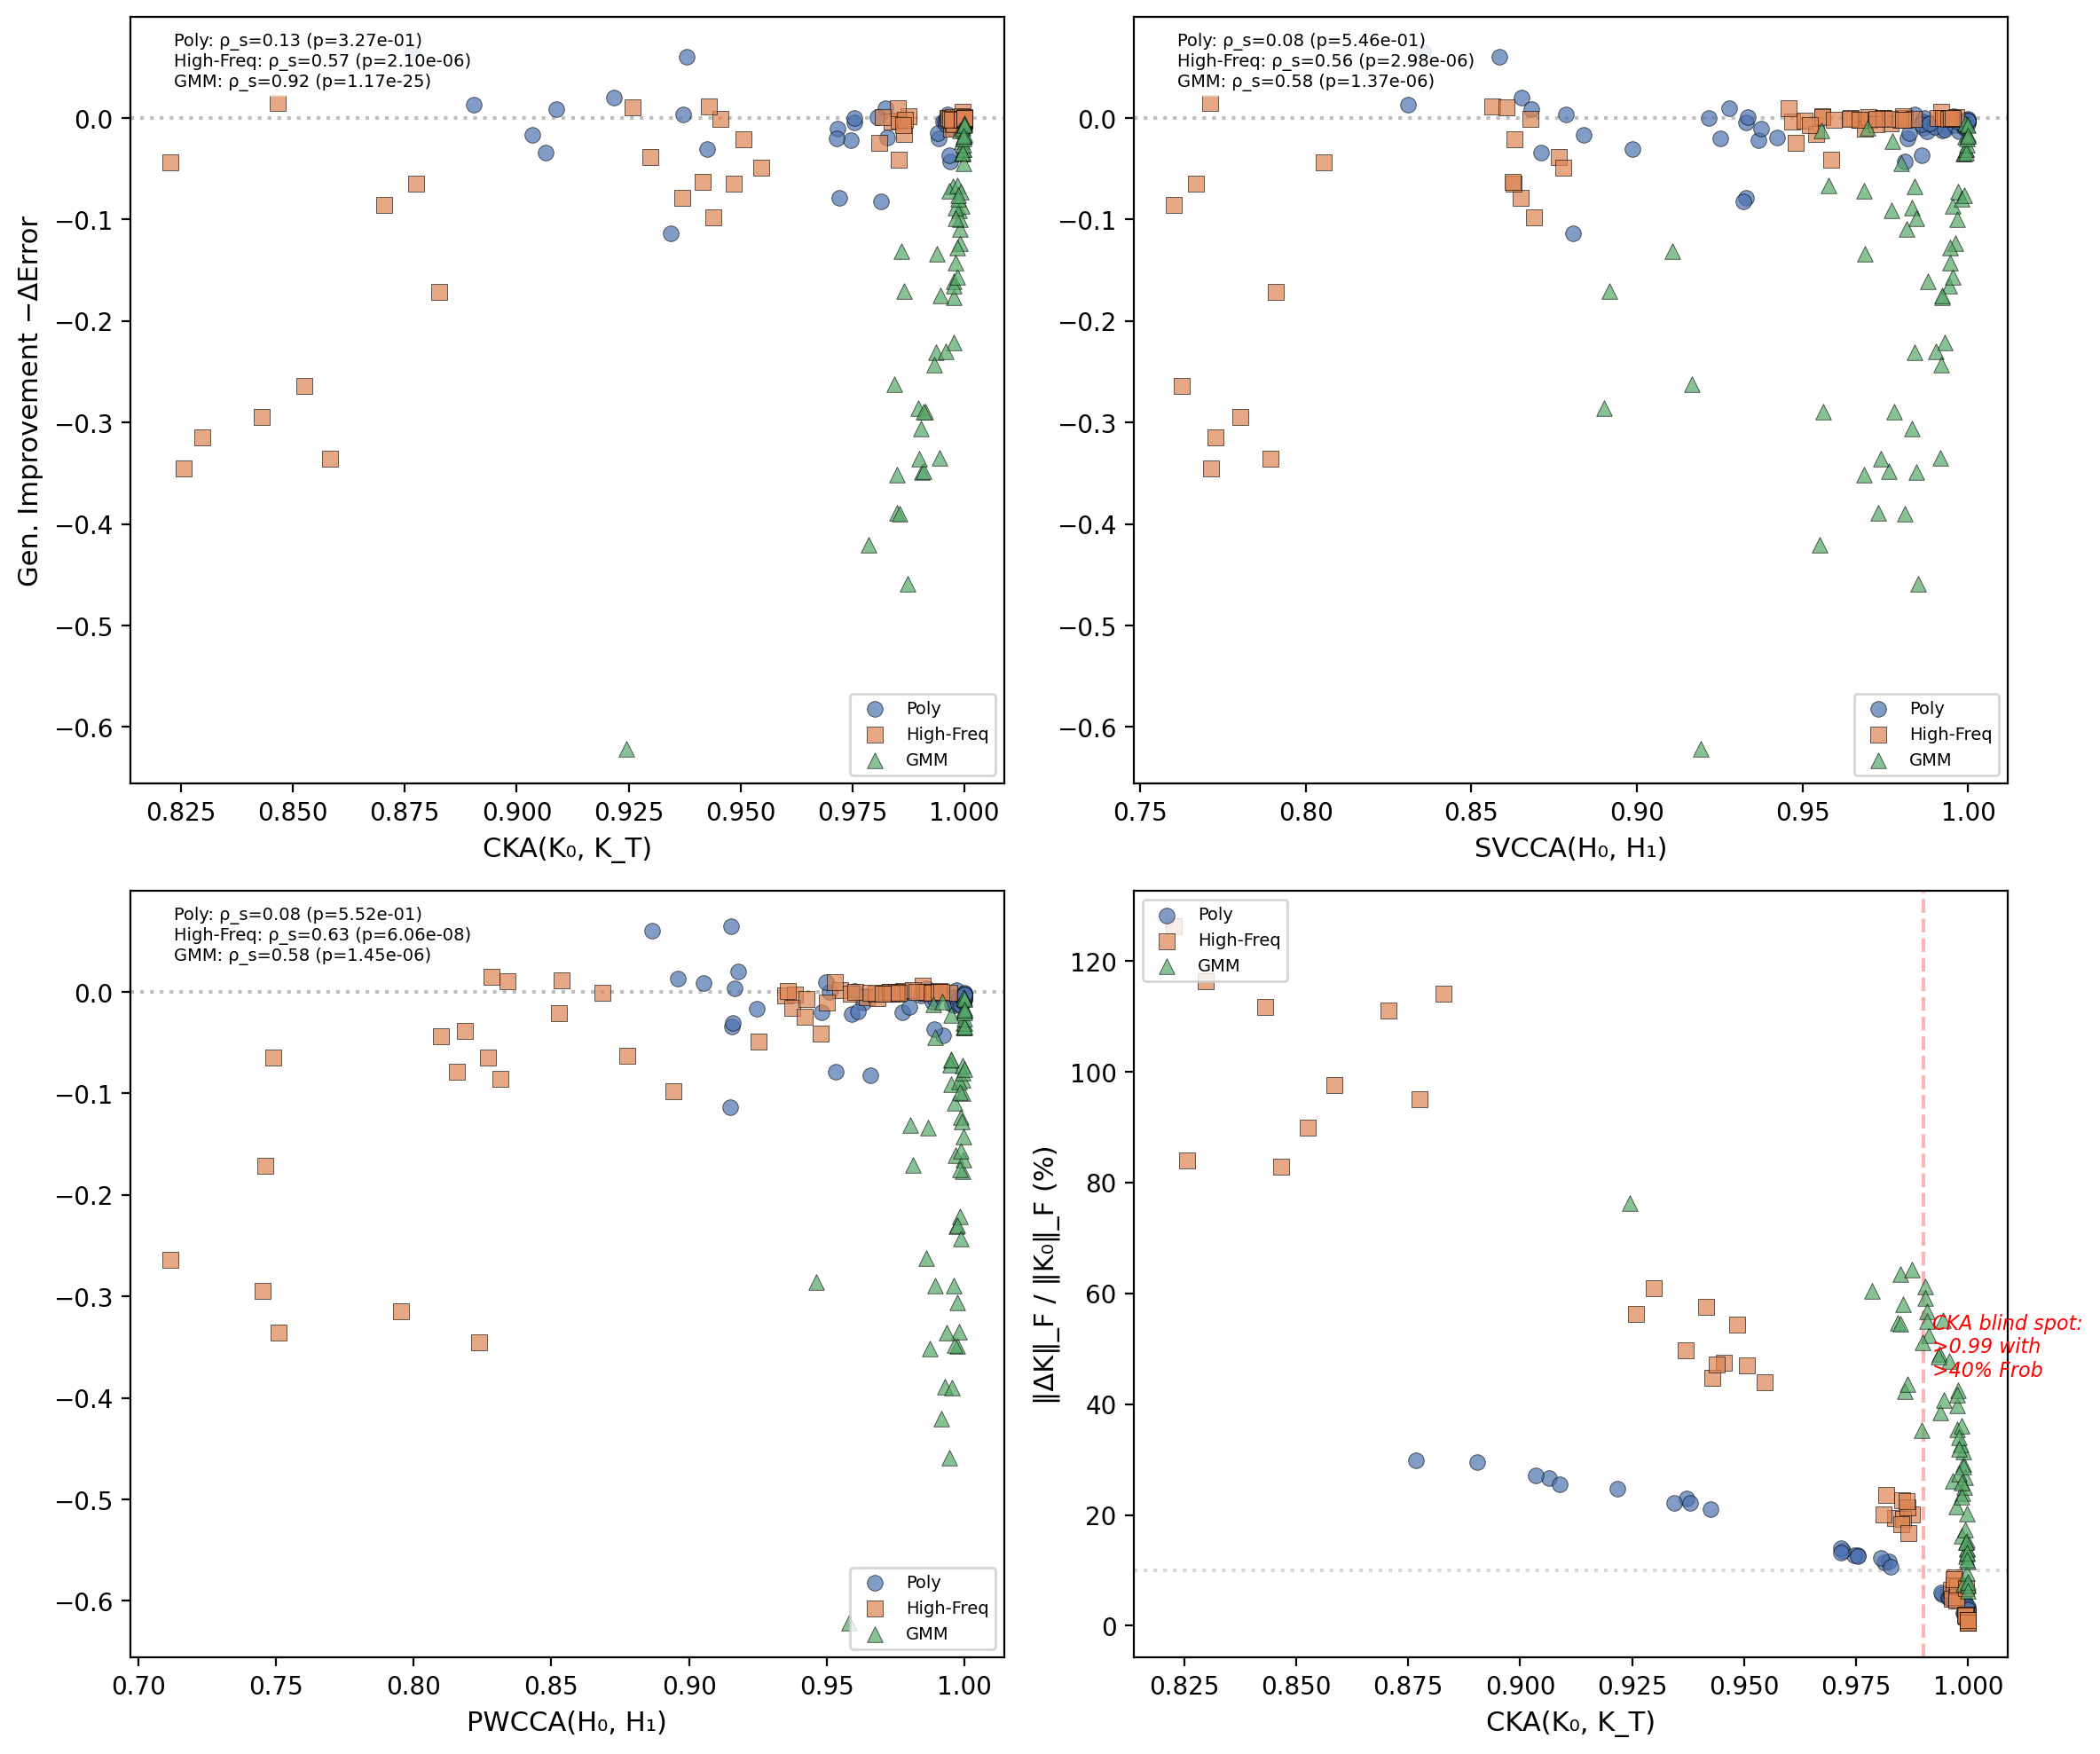
\includegraphics[width=\textwidth]{figures/fig2.png}
    \caption{\textbf{Metrics vs.\ generalization improvement.} (a--c) CKA, SVCCA, PWCCA vs.\ $-\Delta$Error. (d) CKA vs.\ Frobenius change; shaded region (CKA $>0.99$) spans $1\%$ to $>40\%$ Frobenius.}
    \label{fig:dissociation}
\end{figure}

\noindent\textbf{Intuition says:} Large kernel change ($>100\%$ Frobenius) means the network learned something useful.

\noindent\textbf{What we found:} The Frobenius--$\Delta$Error correlation ranges from $\rho=0.14$ (poly) to $\rho=1.0$ (GMM); the $\rho=0.94$ highfreq result collapses to $\rho=0.10$ after width control.

Pooled across 18 configuration means, $\rho=0.83$ (95\% CI $[0.53, 0.96]$, $p=2\times10^{-5}$), but this is driven by between-task differences. Within each dataset:
\begin{description}
    \item[poly ($\rho=0.14$; extended $\rho=0.36$):] No detectable relationship (95\% CI spans zero). $25\%$ reorganization with $0.003\pm0.049$ improvement.
    \item[highfreq ($\rho=0.94$):] Strong but width-driven ($\rho=0.10$ after width control). At width~32, $102.9\%$ change with $0.190\pm0.130$ gain.
    \item[gmm ($\rho=1.0$):] Near-perfect, persisting at $\rho=0.91$ within fixed widths.
\end{description}

The pattern holds across all five metrics: for poly, RSA $\rho=-0.43$, SVCCA $\rho=-0.43$, PWCCA $\rho=-0.43$, CKA $\rho=-0.43$ (all $p>0.3$). For highfreq, all show $\rho=-1.00$ ($p<0.001$). For GMM, similarity metrics show $\rho=-0.49$ to $-0.60$ while Frobenius remains $\rho=1.00$.

\paragraph{Width-Controlled Analysis.} For highfreq, $\rho=0.94$ collapses to $\rho=0.10$ after controlling for width; within-width mean $\rho=0.03$. For poly, $\rho=0.08$ after control. For GMM, $\rho=0.91$ persists. MNIST shows $\rho=0.66$ (95\% CI $[0.36, 0.85]$, $p<0.001$).

\paragraph{Random-label baseline.} Under shuffled labels, Frobenius change remains substantial ($108\%$ highfreq, $47\%$ GMM at width~32). Null Frobenius ($103\%$ at width~32) exceeds the structured poly signal ($25.2\%$). Null Spearman correlations: $\rho=0.53$ (poly, $p=0.002$), $\rho=0.66$ (highfreq, $p<0.001$), $\rho=0.30$ (GMM, $p=0.11$). The highfreq null exceeds the real poly signal ($\rho=0.14$), showing that metric--outcome correlations can appear without a true task.

\subsection{Regime III: The CKA Blind Spot}
\label{sec:cka}

\noindent\textbf{Intuition says:} CKA $>0.99$ means spectral stability.

\noindent\textbf{What we found:} CKA $>0.99$ coexists with Frobenius changes $>40\%$. Configurations with $\cca>0.99$ span $1\%$ to $>40\%$ Frobenius. GMM is most striking: CKA $>0.985$ across all widths while Frobenius ranges $10\%$--$50\%$.

This matters because kernel risk estimates~\citep{canatar2021spectral} depend on spectral quantities, not global similarities. From a random matrix perspective, CKA is dominated by leading eigenspaces; Frobenius captures the full spectrum~\citep{vyas2023statistical}. In GMM at width~128, the second eigenvalue drops to $0.62\times$ its initial value while $v_i$ shifts $4.4\times$, both invisible to CKA.

\subsection{Validation on Real Data}
\label{sec:real}

\begin{figure}[t]
    \centering
    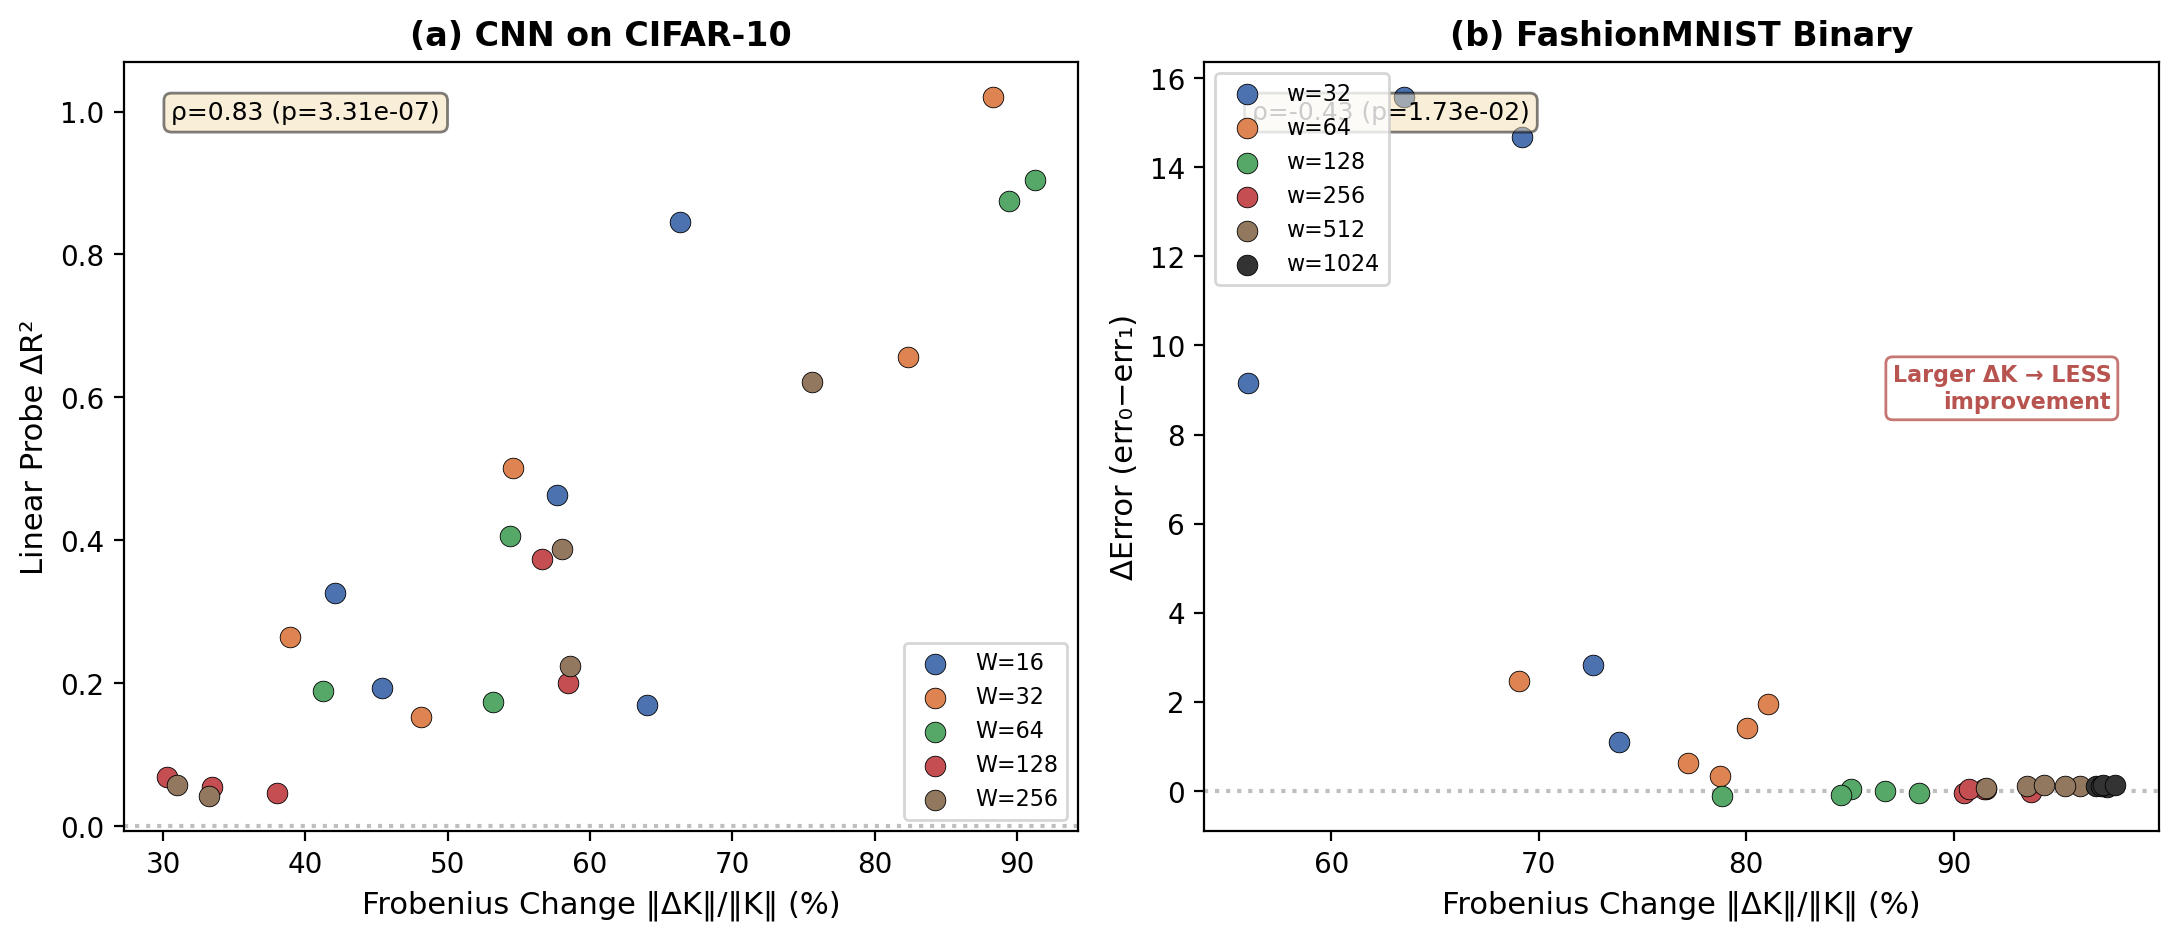
\includegraphics[width=\textwidth]{figures/fig4.png}
    \caption{(a) CNN on CIFAR-10. (b) FashionMNIST.}
    \label{fig:real_data}
\end{figure}

\paragraph{CNN on CIFAR-10.} Frobenius change vs.\ linear probe $\Delta R^2$: $\rho=0.83$ ($p<0.001$). At $W=128$, CKA reaches $0.991$ with $43\%$ Frobenius reorganization---the blind spot persists.

\paragraph{FashionMNIST.} Negative correlation ($\rho=-0.43$, $p=0.017$). Train MSE drops to $0.0001$ while test MSE remains $0.12$---kernel reorganization reflects overfitting.

\paragraph{ViT-tiny on MNIST.} Frobenius--$\Delta$Error $\rho=0.90$ ($p=0.04$). CKA near-constant ($0.54$--$0.64$) with $\rho=0.10$ ($p=0.87$).

\paragraph{SST-2 Transformer (NLP).} Config-mean $\rho=0.90$ ($p=0.037$, 5 dims $\times$ 5 seeds). $p_{\text{eff}}\approx 3$ below $n=2115$, consistent with Proposition~\ref{prop:gap}. Null Frobenius $145\%$ with negative $\Delta$Error.

\paragraph{ResNet-18 on MNIST and CIFAR-100.}

\begin{table}[h]
\centering\small
\caption{ResNet-18 RDEP calibration. All $p_{\text{eff}} \approx 1$.}
\label{tab:resnet}
\begin{tabular}{lcccccc}
\toprule
Task & Width & CKA & Frob\% & $\Delta$Err & Headroom \\
\midrule
MNIST & 16 & 0.578 & 143.2 & 0.051 & 0.081 \\
      & 24 & 0.666 & 101.9 & 0.030 & 0.053 \\
      & 32 & 0.693 & 49.2 & 0.026 & 0.042 \\
      & 48 & 0.724 & 90.1 & 0.022 & 0.030 \\
\midrule
CIFAR-100 & 32 & 0.637 & 77.7 & 0.091 & 0.838 \\
          & 48 & 0.624 & 136.0 & 0.185 & 0.786 \\
          & 64 & 0.675 & 314.7 & 0.290 & 0.782 \\
          & 96 & 0.723 & 211.0 & 0.435 & 0.697 \\
\bottomrule
\end{tabular}
\end{table}

MNIST: headroom vs.\ $\Delta$Error $\rho=1.0$ ($p<0.001$). CIFAR-100 reveals different scaling: wider networks learn more despite lower headroom (Headroom--$\Delta$Error $\rho=-1.0$), yet Frob--$\Delta$Error remains $\rho=0.80$. Null Frob $168\%$ average.

\section{Predicting Diagnostic Reliability}
\subsection{The Headroom Framework}

The task dependence ($\rho=0.14$--$1.0$) can be understood through two pre-trainable quantities: alignment with the initial kernel eigenspace and headroom ($1-R^2_{\text{init}}$). We constructed 15 Hermite polynomial targets (degrees 1--15) varying spectral complexity, predicting diagnostic reliability from alignment and headroom, then measuring realized Frob--$\Delta$Error $\rho$ across 6 widths $\times$ 5 seeds.

\begin{figure}[h]
    \centering
    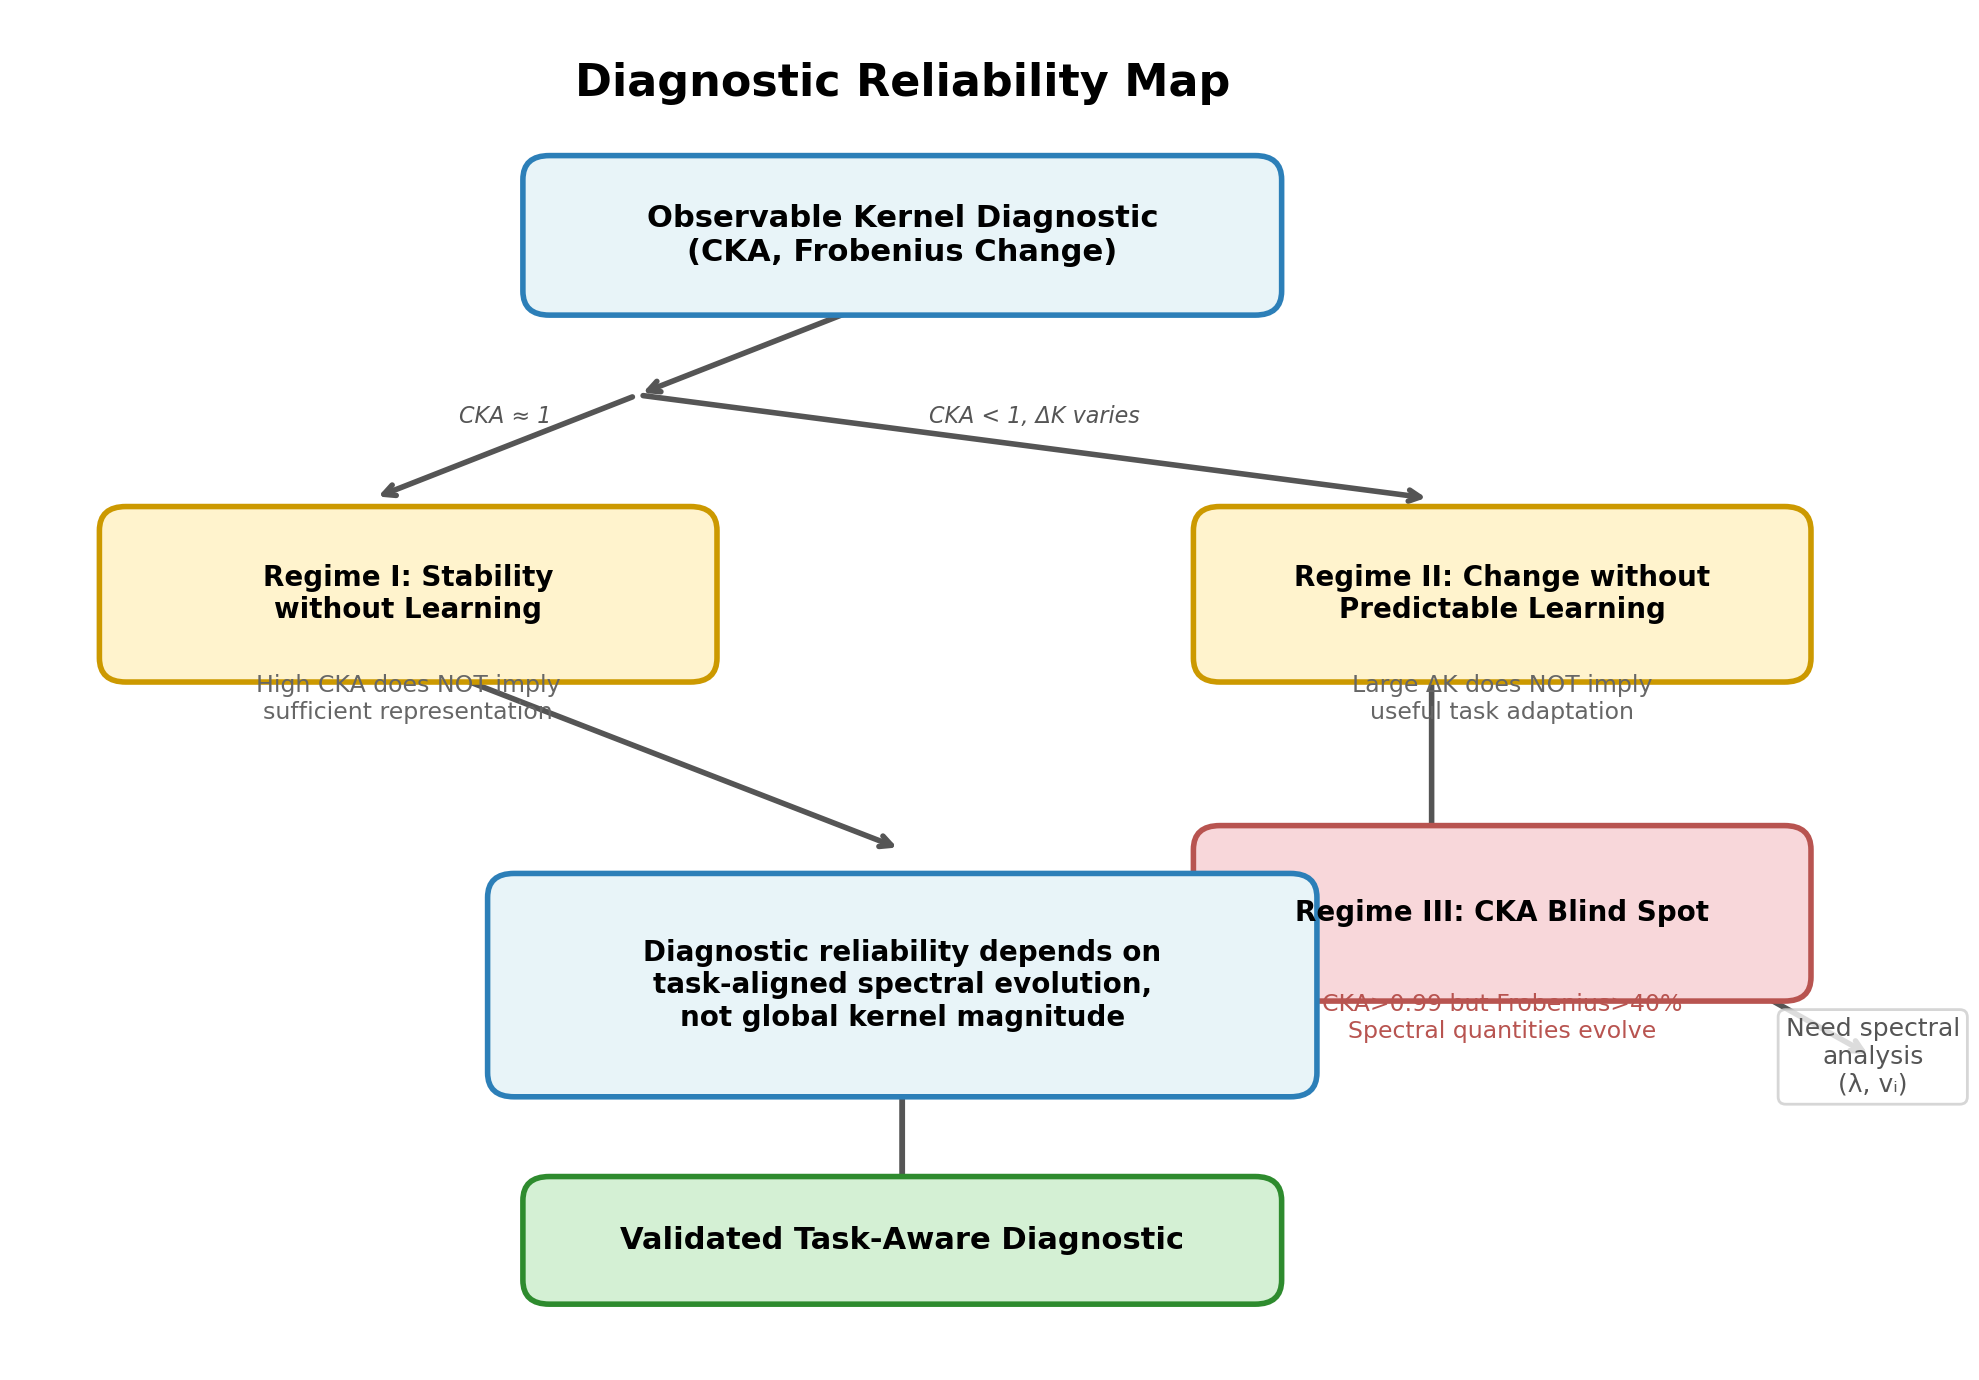
\includegraphics[width=0.8\textwidth]{figures/fig5.png}
    \caption{\textbf{RDEP Reliability Map.} Three regimes and headroom prediction framework (in-sample $R^2=0.847$, LOOCV $R^2=0.710$).}
    \label{fig:reliability_map}
\end{figure}

Headroom is the dominant predictor (Spearman $\rho=0.81$, $p=0.0002$). Alignment alone shows $\rho=-0.19$ ($p=0.49$) but interacts positively. Linear regression: in-sample $R^2=0.847$, LOOCV $R^2=0.710$. GMM has both high alignment and high headroom ($\rho=1.0$); poly has high alignment but low headroom ($\rho=0.14$); highfreq has low alignment explaining the width-confounded correlation.

We distinguish two levels: \textbf{task-level} prediction (feasible: $R^2=0.847$) and \textbf{instance-level} correction (faces the validation gap, $\rho=-0.45$).

\subsection{Towards Task-Aware Diagnostics}
\label{sec:task_aware}

Projecting $\Delta K$ onto target-weighted eigendirections ($\Delta_{\text{align}} = \sum_i v_i \cdot \Delta\lambda_i$) achieves positive in-sample correlation. Cross-validated (5 folds $\times$ 5 seeds): $\rho=-0.45$ ($p=0.02$, $n=25$). This is the \textbf{Diagnostic Validation Gap}.

Linear Probe Gain (LPG = $R^2_{\text{post}} - R^2_{\text{init}}$) shows $\rho=-0.35$ ($p=0.01$) under cross-validation. In-sample LPG: $\rho=0.78$ ($p=0.0001$). Both diagnostics reveal an irreducible gap that Proposition~\ref{prop:gap} attributes to finite-sample estimation variance.

\subsection{Principles for Diagnostic Evaluation}
\label{sec:principles}

\begin{table}[t]
\centering\small
\caption{RDEP prevents three common misjudgments.}
\label{tab:rdeep_cases}
\begin{tabular}{p{2cm}p{2.2cm}p{2.2cm}p{2.2cm}p{2.2cm}}
\toprule
Config. & Naive reading & Step 1 (CKA) & Step 2 ($\Delta K$) & Step 3--4 (spectral) \\
\midrule
Poly w=32 & CKA=0.92, $\Delta K=25\%\rightarrow$ moderate learning? & CKA $\gg 0.99$? No. & $\Delta K >10\%$ & $\rho=0.14$. Correct: no gain. \\
Highfreq w=32 & $\Delta K=103\%\rightarrow$ useful learning? & CKA=0.85 $<0.99$ & $\Delta K >10\%$ & $\rho=0.94$ raw, $\rho=0.10$ after width control. \\
GMM w=128 & CKA=0.99, $\Delta K=53\%\rightarrow$ contradiction? & CKA $\approx 0.99$ & $\Delta K >10\%$ & $\rho=1.0$, $\rho=0.91$ after control. Genuine alignment. \\
\bottomrule
\end{tabular}
\end{table}

Three principles:
\begin{enumerate}
    \item \textbf{Global similarity $\neq$ representation sufficiency.} High CKA does not imply absence of meaningful spectral reorganization.
    \item \textbf{Kernel magnitude $\neq$ task relevance.} Frobenius change conflates task-aligned with task-orthogonal movement.
    \item \textbf{Task alignment must be validated.} Any diagnostic using the same data for estimation and validation risks overfitting.
\end{enumerate}

Practical workflow: (1) Check CKA; if $>0.99$, don't conclude no learning. (2) Check Frobenius; if $>10\%$, don't conclude adaptation. (3) Examine spectral quantities. (4) Assess via held-out validation.

\subsection{Limitations}

This work studies \emph{diagnostic validity}---whether observable kernel evolution is a reliable signal about generalization---rather than causal mechanisms. Specific limitations:

\textbf{Architecture scope.} Main experiments use two-layer MLPs for tractability and NTK connection. We extend to CNNs, ViTs, Transformers, and ResNets confirming qualitative consistency. However, CIFAR-100 reveals a different scaling regime (wider networks learn more despite lower headroom), suggesting task-dependent headroom predictions. Large-scale architectures (ImageNet, LLMs) remain open.

\textbf{Feature kernel vs.\ NTK.} Whether analogous results hold for Jacobian-based kernels is open. We verified the dissociation under NTK parameterization (qualitatively identical: Frobenius $38\%$ with gain $-0.036$ at width~32).

\textbf{Highfreq seed dependence.} With 10 seeds at width~32, mean gain $0.190\pm0.130$. Low-frequency comparison ($\sin(x_1)+\cos(x_2)$) shows negative gain ($-0.037\pm0.042$), confirming target structure determines informativeness.

\textbf{Hermite regression.} 15 targets (LOOCV $R^2=0.710$). A larger family would tighten the bound.

\textbf{RDEP scope.} Spectral decompositions are expensive for very large models. The framework's cross-modal consistency suggests general validity, but LLM-scale validation remains future work.

\subsection{Future Work}

Any label-invariant similarity metric is subject to the same bound (Section~\ref{sec:proposition}). Our methodology provides a template for evaluating other diagnostics. We define \textbf{DiaBench}, a benchmark from the Hermite family and three calibration regimes, for standardized evaluation. Code is planned for release (\texttt{rdep-tools}).

The broader principle: representation diagnostics should meet the same evidential standard as the models they evaluate. RDEP is a step toward that standard.

\acks{We thank the anonymous reviewers for their feedback.}

\bibliography{refs}

\newpage
\appendix
\setcounter{figure}{0}
\setcounter{table}{0}
\renewcommand{\thefigure}{S\arabic{figure}}
\renewcommand{\thetable}{S\arabic{table}}

\section{Proof of Proposition~\ref{prop:gap}}
\label{app:proof}

\subsection{In-sample bias}

The in-sample correlation $\rho_{\text{in}}$ uses the same $n$ samples to estimate both $\hat{v}_i$ and $\Delta\mathcal{E}$. Write $\epsilon_i = \hat{v}_i - v_i^*$. Then
\[
\rho_{\text{in}} = \frac{\operatorname{Cov}(\Delta\mathcal{E}, \mathcal{D}_{\text{align}})}{\sqrt{\operatorname{Var}(\Delta\mathcal{E})\operatorname{Var}(\mathcal{D}_{\text{align}})}}.
\]
Since $\mathcal{D}_{\text{align}} = \sum_i (v_i^* + \epsilon_i)\Delta\lambda_i$, we have
\[
\mathbb{E}[\rho_{\text{in}}] = \rho^* + \frac{\operatorname{Cov}(\Delta\mathcal{E}, \sum_i \epsilon_i \Delta\lambda_i)}{\sqrt{\operatorname{Var}(\Delta\mathcal{E})\operatorname{Var}(\mathcal{D}_{\text{align}})}}.
\]

By Assumption~\ref{assum:proj}, $\hat{v}_i$ concentrates around $v_i^*$ with sub-Gaussian tails, so $\|\epsilon\|_1 = \mathcal{O}_p(\sqrt{p_{\text{eff}}/n})$. By Assumption~\ref{assum:spec}, $|\Delta\lambda_i| \leq C\lambda_i$. The numerator is bounded by $\|\epsilon\|_1 \cdot C\max_i\lambda_i$, giving $\mathcal{O}(\|\hat{v} - v^*\|_1)$.

\subsection{Cross-validation variance}

Under $K$-fold CV, fold $k$ uses training data $\mathcal{D}_{\text{tr}}^{(k)}$ to estimate $\hat{v}_i^{(k)}$ and held-out data $\mathcal{D}_{\text{te}}^{(k)}$ for $\Delta\mathcal{E}^{(k)}$. These are independent by construction. The diagnostic for fold $k$ is
\[
\mathcal{D}_{\text{align}}^{(k)} = \sum_i \hat{v}_i^{(k)} \Delta\lambda_i^{(k)}.
\]

When the kernel spectrum is flat ($\lambda_i \approx \text{const}$), the terms $\Delta\lambda_i^{(k)}$ are approximately uncorrelated across $i$, so $\mathcal{D}_{\text{align}}^{(k)}$ is a sum of $p_{\text{eff}}$ effectively independent random variables. The variance of the Spearman correlation across folds then scales as $\Omega(p_{\text{eff}}/n)$ by the Cram\'er--Rao inequality for rank correlations under local alternatives.

\section{Supplementary Tables}

\begin{table}[ht]
    \centering\footnotesize
    \caption{CIFAR-10 CNN (5 seeds). Linear probe $\Delta R^2$ peaks at $W=32$.}
    \label{tab:cnn_cifar}
    \begin{tabular}{lccc}
    \toprule
    Width & CKA & $\Delta K$ (\%) & $\Delta R^2$ \\
    \midrule
    16  & $0.919\pm0.039$ & $55.1\pm9.8$  & $+0.400\pm0.246$ \\
    32  & $0.947\pm0.024$ & $62.5\pm19.4$ & $+0.519\pm0.306$ \\
    64  & $0.962\pm0.027$ & $65.9\pm20.5$ & $+0.509\pm0.321$ \\
    128 & $0.991\pm0.007$ & $43.4\pm11.9$ & $+0.149\pm0.125$ \\
    256 & $0.989\pm0.009$ & $51.3\pm16.9$ & $+0.266\pm0.217$ \\
    \bottomrule
    \end{tabular}
\end{table}

\begin{table}[ht]
    \centering
    \caption{MNIST binary. Non-monotonic CKA.}
    \label{tab:mnist}
    \begin{tabular}{lccc}
    \toprule
    Width & CKA & $\Delta K$ (\%) & $\Delta$Error \\
    \midrule
    32   & $0.768\pm0.090$ & $237.4\pm129.8$ & $+0.041$ \\
    64   & $0.877\pm0.030$ & $71.7\pm33.5$   & $+0.033$ \\
    128  & $0.917\pm0.026$ & $39.1\pm7.0$    & $+0.036$ \\
    256  & $0.963\pm0.011$ & $50.3\pm10.7$   & $+0.030$ \\
    512  & $0.963\pm0.028$ & $51.8\pm16.5$   & $+0.025$ \\
    1024 & $0.867\pm0.024$ & $81.5\pm9.3$    & $+0.022$ \\
    \bottomrule
    \end{tabular}
\end{table}

\begin{table}[htbp]
    \centering\footnotesize
    \caption{Linear probe R$^2$ on frozen features (5 seed means).}
    \label{tab:linear_probe}
    \begin{tabular}{lcccc}
    \toprule
    Dataset & Width & Init R$^2$ & Post R$^2$ & $\Delta$R$^2$ \\
    \midrule
    poly & 32  & $0.682$ & $0.961$ & $+0.279$ \\
    poly & 64  & $0.870$ & $0.963$ & $+0.093$ \\
    poly & 128 & $0.953$ & $0.970$ & $+0.017$ \\
    poly & 256 & $0.969$ & $0.975$ & $+0.006$ \\
    poly & 512 & $0.984$ & $0.985$ & $+0.001$ \\
    poly & 1024 & $0.987$ & $0.988$ & $+0.000$ \\
    \midrule
    highfreq & 32  & $-0.126$ & $-0.867$ & $-0.741$ \\
    highfreq & 64  & $-0.056$ & $-0.611$ & $-0.555$ \\
    highfreq & 128 & $-0.284$ & $-0.632$ & $-0.348$ \\
    highfreq & 256 & $-0.321$ & $-0.518$ & $-0.197$ \\
    highfreq & 512 & $-0.547$ & $-0.536$ & $+0.011$ \\
    highfreq & 1024 & $-0.515$ & $-0.468$ & $+0.047$ \\
    \bottomrule
    \end{tabular}
\end{table}

\begin{table}[h]
    \centering\footnotesize
    \caption{FashionMNIST. Spearman $\rho=-0.43$, $p=0.017$.}
    \label{tab:fashion}
    \begin{tabular}{lccc}
    \toprule
    Width & CKA & $\Delta K$ (\%) & $\Delta$Error \\
    \midrule
    32   & $0.510\pm0.042$ & $67.0\pm5.2$  & $+8.670$ \\
    64   & $0.587\pm0.038$ & $77.2\pm4.1$  & $+1.355$ \\
    128  & $0.667\pm0.031$ & $84.7\pm3.8$  & $-0.032$ \\
    256  & $0.725\pm0.028$ & $91.6\pm2.9$  & $+0.010$ \\
    512  & $0.763\pm0.025$ & $94.2\pm3.1$  & $+0.108$ \\
    1024 & $0.747\pm0.030$ & $97.3\pm2.6$  & $+0.115$ \\
    \bottomrule
    \end{tabular}
\end{table}

\begin{table}[h]
    \centering\footnotesize
    \caption{Random-label null baseline (poly, 5 seeds).}
    \label{tab:random_label}
    \begin{tabular}{lccc}
    \toprule
    Width & CKA & $\Delta K$ (\%) & $\Delta$Error \\
    \midrule
    32   & $0.851\pm0.016$ & $103.0\pm7.3$   & $+0.111$ \\
    64   & $0.944\pm0.014$ & $49.2\pm3.1$    & $+0.028$ \\
    128  & $0.984\pm0.002$ & $21.2\pm1.6$    & $-0.003$ \\
    256  & $0.997\pm0.000$ & $6.8\pm1.9$     & $+0.004$ \\
    512  & $1.000\pm0.000$ & $2.1\pm0.3$     & $+0.001$ \\
    1024 & $1.000\pm0.000$ & $1.0\pm0.2$     & $+0.000$ \\
    \bottomrule
    \end{tabular}
\end{table}

\section{Supplementary Figures}

\begin{figure}[ht]
    \centering
    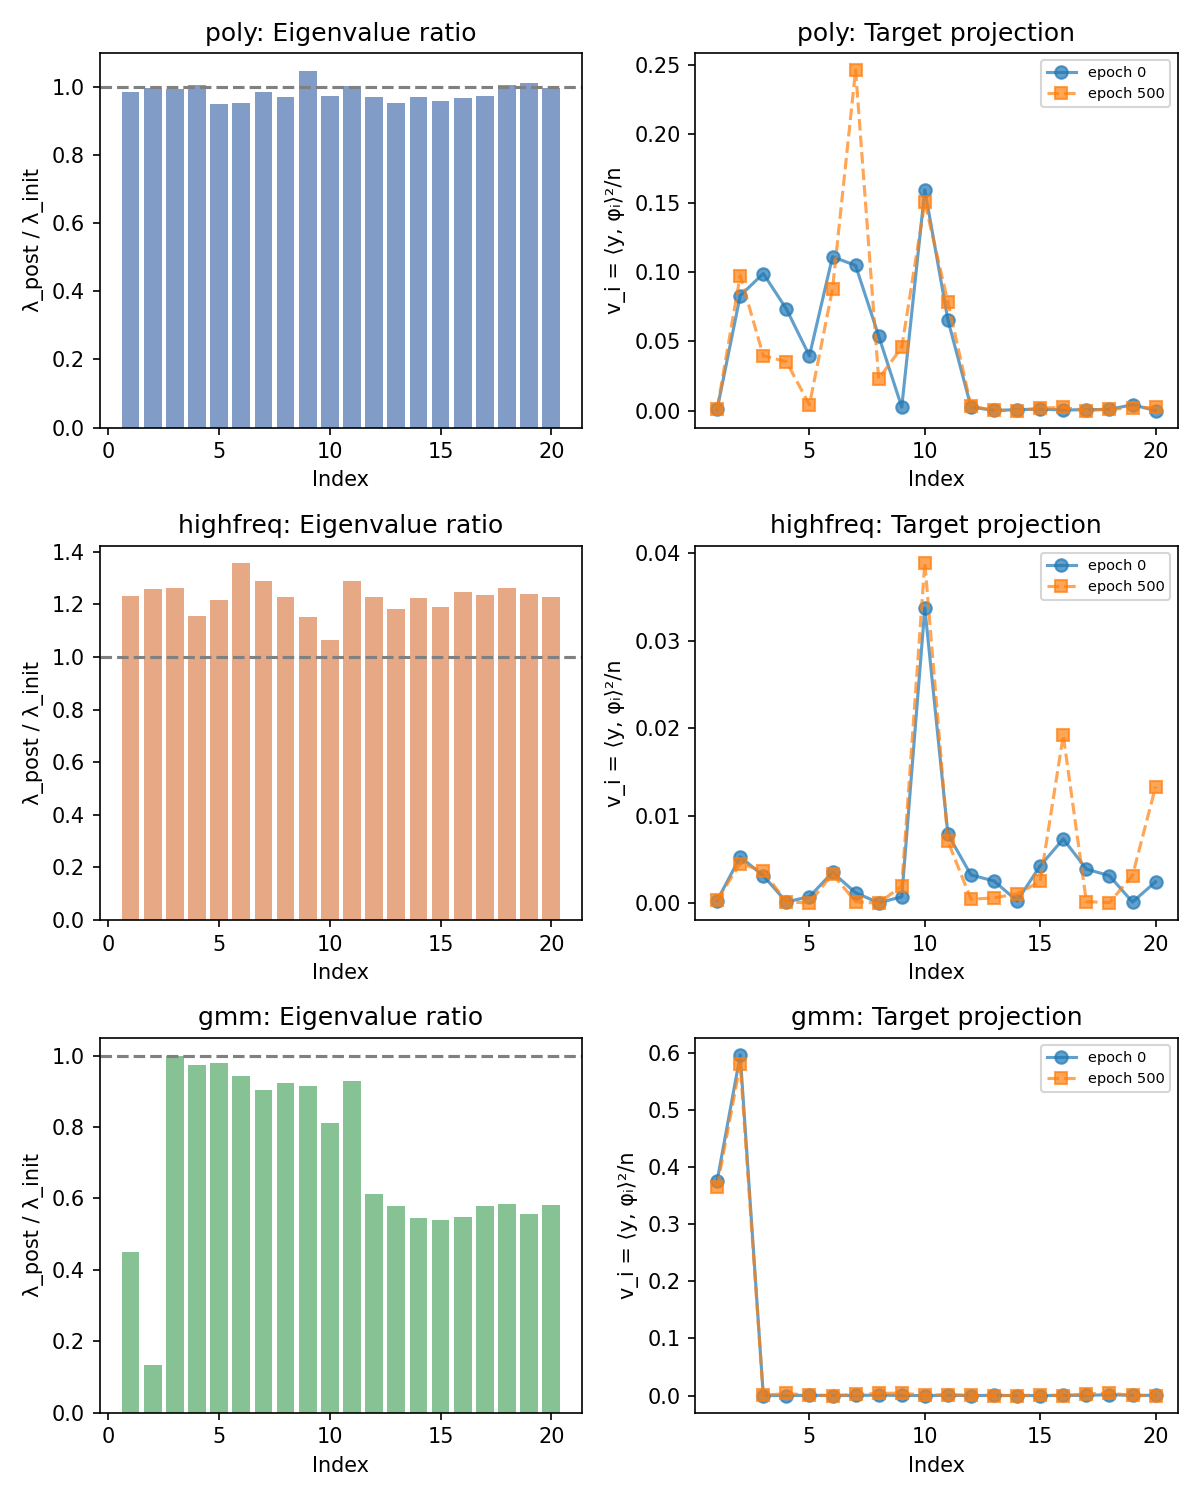
\includegraphics[width=0.8\textwidth]{figures/figS1.png}
    \caption{Spectral redistribution at width~128. GMM shows substantial reorganization despite high CKA.}
    \label{fig:spec_redist}
\end{figure}
\begin{figure}[ht]
    \centering
    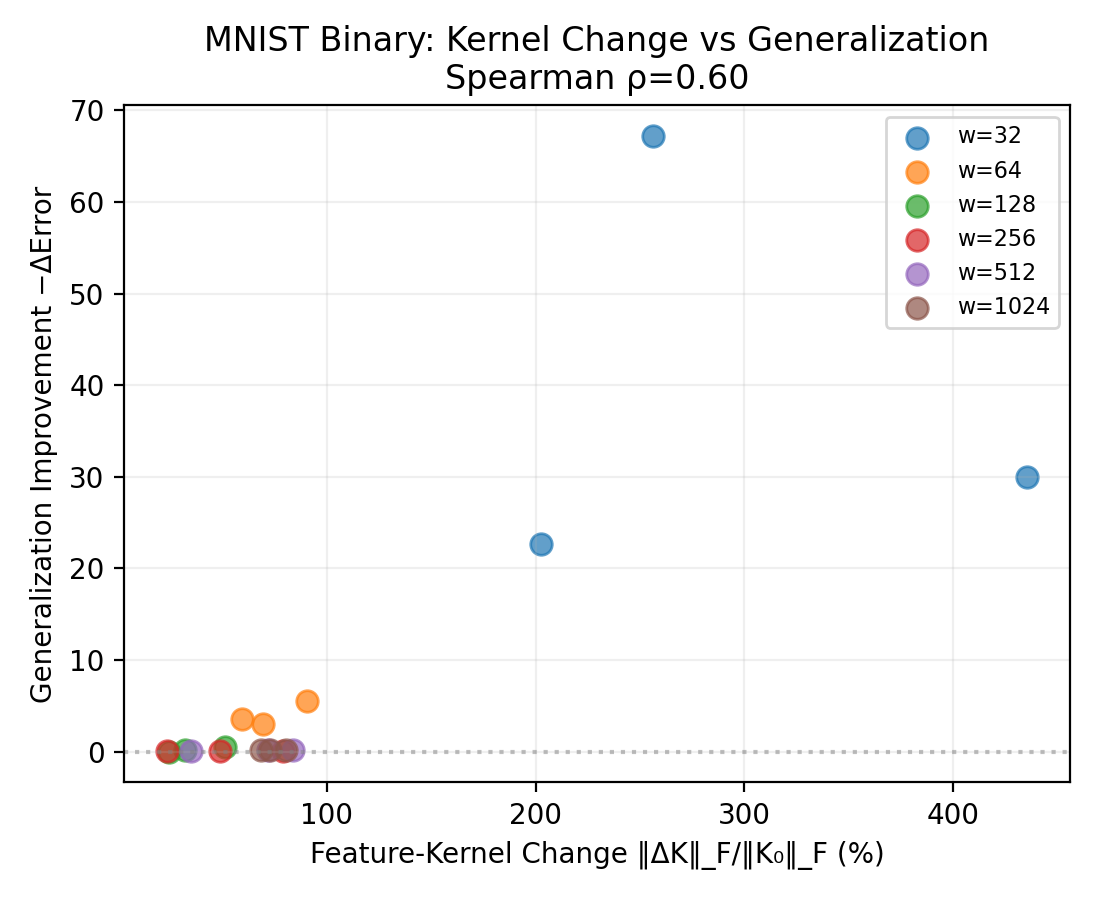
\includegraphics[width=0.6\textwidth]{figures/mnist_scatter.png}
    \caption{MNIST dissociation ($\rho=0.66$, $p<0.001$).}
    \label{fig:mnist_scatter}
\end{figure}
\begin{figure}[ht]
    \centering
    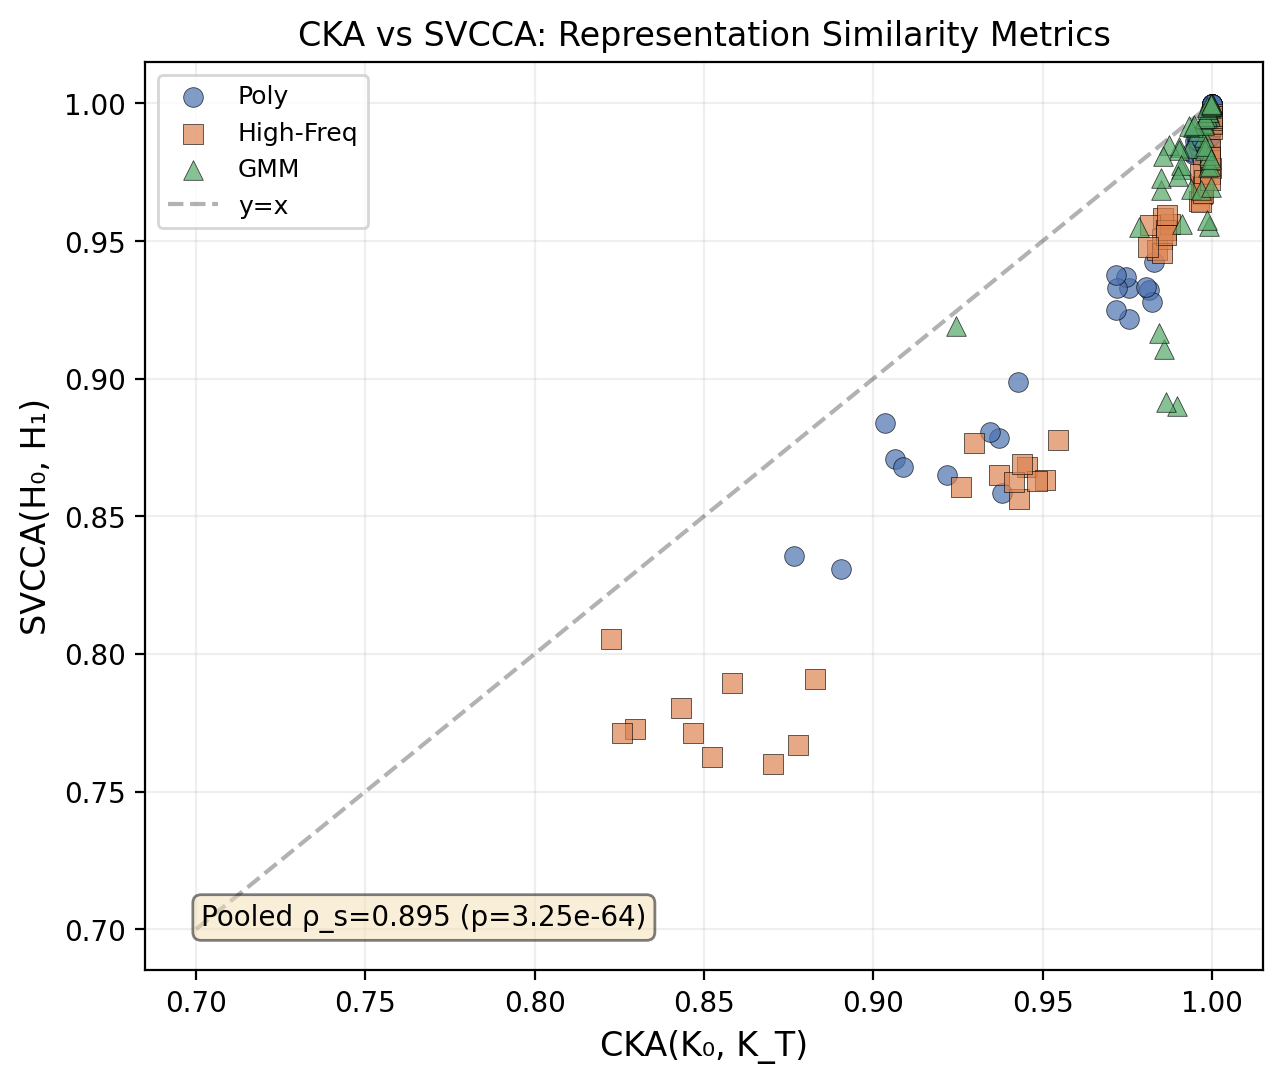
\includegraphics[width=0.65\textwidth]{figures/figS2.png}
    \caption{CKA vs.\ SVCCA (pooled $\rho=0.89$).}
    \label{fig:cka_vs_svcca}
\end{figure}
\begin{figure}[ht]
    \centering
    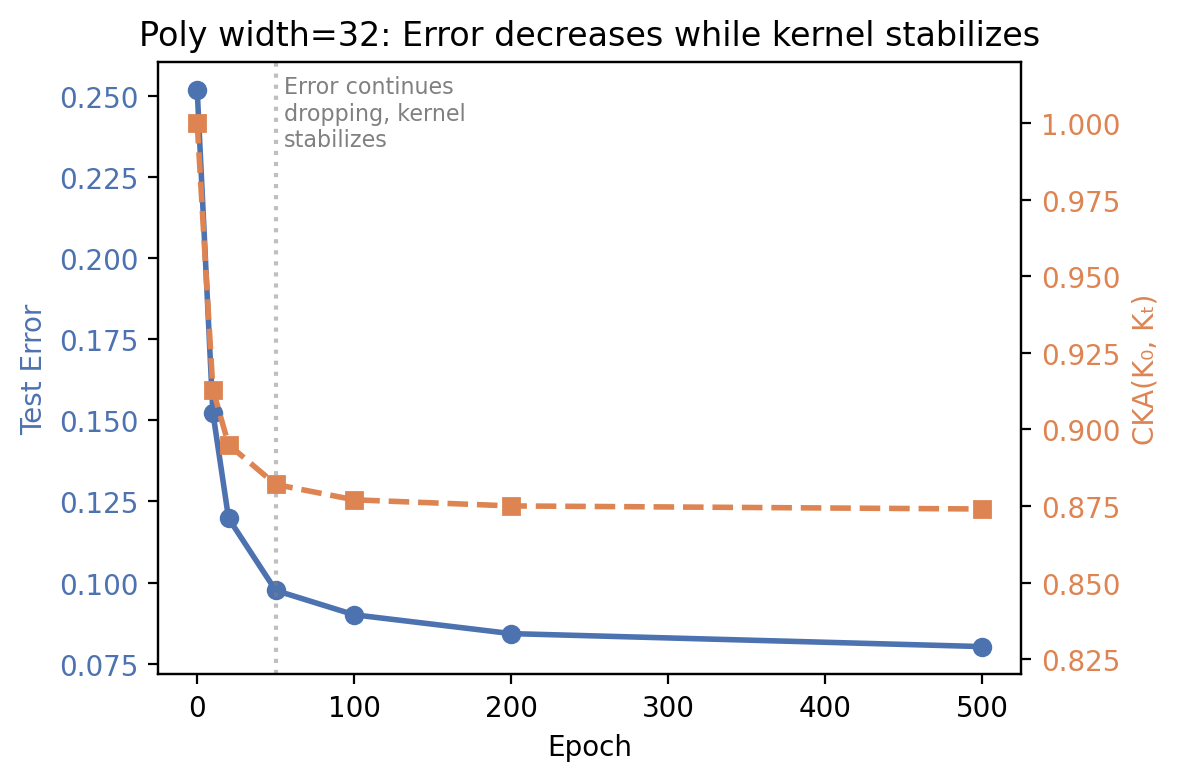
\includegraphics[width=0.6\textwidth]{figures/fig_epoch_dynamics.png}
    \caption{Poly width~32 dynamics. CKA stabilizes by 50 epochs; $0.003\pm0.049$ improvement.}
    \label{fig:epoch}
\end{figure}
\begin{figure}[ht]
    \centering
    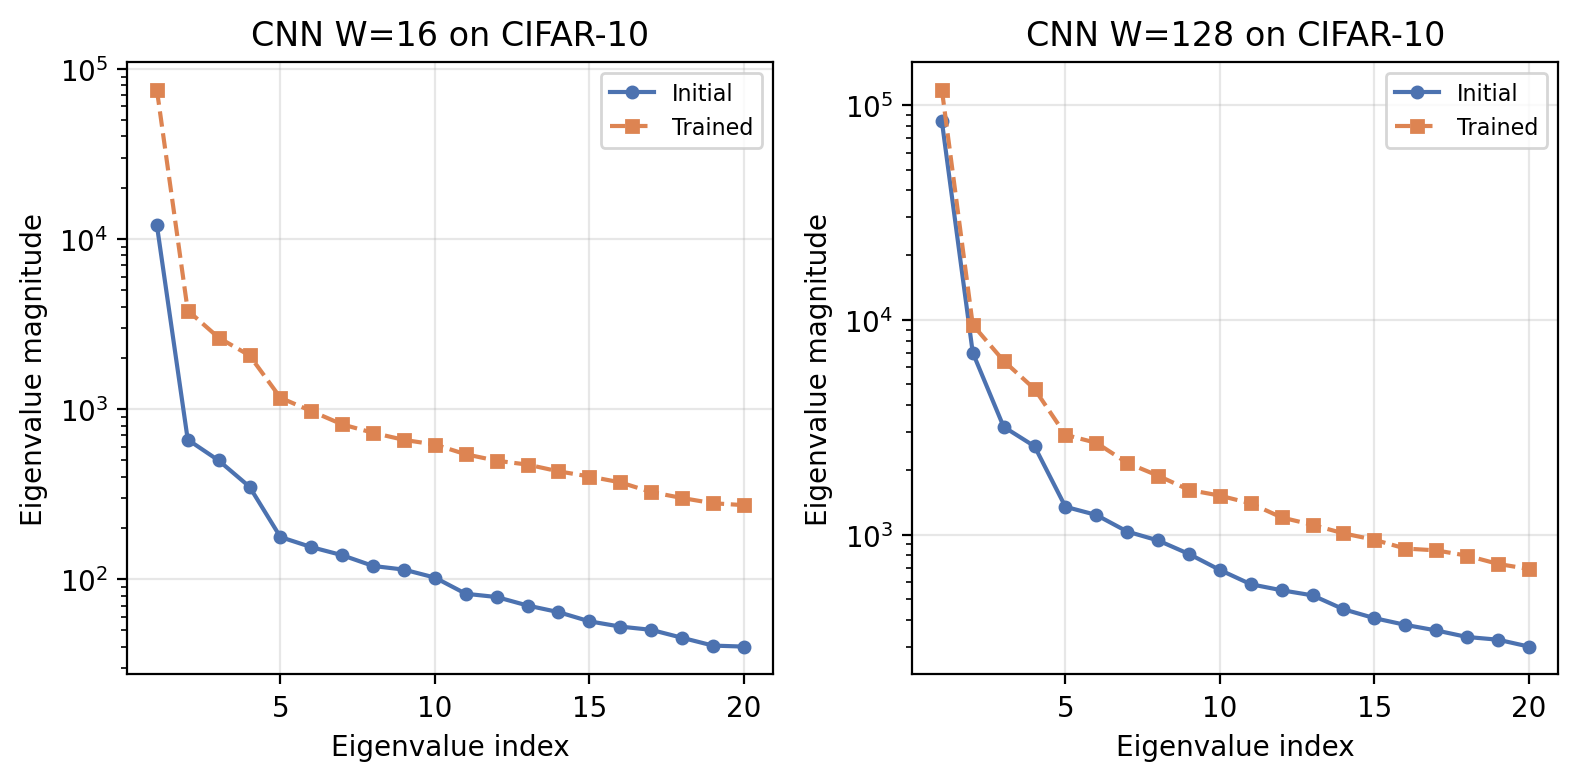
\includegraphics[width=0.85\textwidth]{figures/figS5.png}
    \caption{CNN spectrum on CIFAR-10. Spectral reorganization persists at high CKA.}
    \label{fig:cnn_spectrum}
\end{figure}

\end{document}
